
\addcontentsline{toc}{section}{Введение}






\section*{Введение}\label{intro}

Индуцирование плазмонного резонанса в системе с напылением проводящего слоя на диэлектрики различной конфигурации (призма или цилиндр ) открывают возможность создать очень чувствительный к внешним параметрам сенсор.

\begin{figure}[h!]
	\centering
	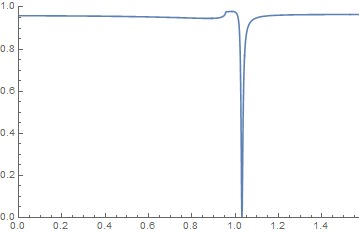
\includegraphics[width=0.5\linewidth]{kretchmann}
	\caption{Эффект Кречмана}\label{fig:kretchmann}
\end{figure}



Физическое явление которое легло в основание данной схемы было предложено Кречманом и Отто. Для производства сенсоров наиболее применимой и удобной является схема Кречмана которая является фундаментом для построения схемы расмотренной в данной работе.
Световой пучок падает на ~\ref{fig:sandwitch} сэндвич из диэлектрика с $ \varepsilon_p >1 $ и слоя с металлическим напылением испытывая полное внутренне отражаение. В идеалированной ситуации коэффицент отражения равен единице, однако при некотором угле падение возникает резкое падение ~\ref{fig:kretchmann}коэффицента отражения вызванное скачком интенсивности поля у металла. В литературе это называют нарушенным полным внутренним отражением (НПВО).

Данная конфигурация очень полезна так-как позволяет посчитать $ \varepsilon $ среды граничащей с металлом по расположению скачка коэффицента отражения из-за чувствительности данной схемы к свойствам материала.

В данной же работе будет исследована цилиндрическая конфигурация с наклонной брегговской решёткой.


\begin{center}
	\begin{figure}[h]
		\centering
		\begin{tikzpicture}
		
		\node[] at (60:1.5)  {$\theta$};
		\node[] at (35:1)  {$\alpha$};
		\node[] at (12:6.2)  {$\beta$};
		\coordinate (fov) at (2, 1);
		
		\draw[thick,blue, snake=coil,segment aspect=0.15] (fov) -- ++(220:1.5cm);
		\draw[thick,red, snake=coil,segment aspect=0.15] (fov) -- ++(150:3cm);
		\draw[thick,green, snake=coil,segment aspect=0.15] (5,1) -- ++(30:2cm);
		
		\draw[thick] (1,1) arc (180:215:1) ;
		\draw[thick] (0.9,1) arc (180:150:1) ;
		\draw[thick] (5.7,1) arc (0:30:0.6) ;
		\draw[thick,->](8,1) -- (-1,1)  ;
		
		
		\definecolor{color1}{RGB}{252,156,12};
		\definecolor{color2}{RGB}{252,124,12};
		\definecolor{color3}{RGB}{252,104,12};
		\fill[fill=color1,opacity=.7]  (2,0) rectangle (3,2) ;
		\fill[fill=color2,opacity=.7]  (3,0) rectangle (4,2) ;
		\fill[fill=color3,opacity=.7]  (4,0) rectangle (5,2) ;
		\end{tikzpicture}
		\caption{Трёхслойная среда с показателями преломления $ n_1, n_2, n_3 $}\label{fig:sandwitch}
	\end{figure}
	
	
\end{center}





